\chapter{User Study Results}\label{chapter:experiment_results}
\section{Results Interpretion}
\subsection{Duration}
\begin{figure}[h]
    \centering
    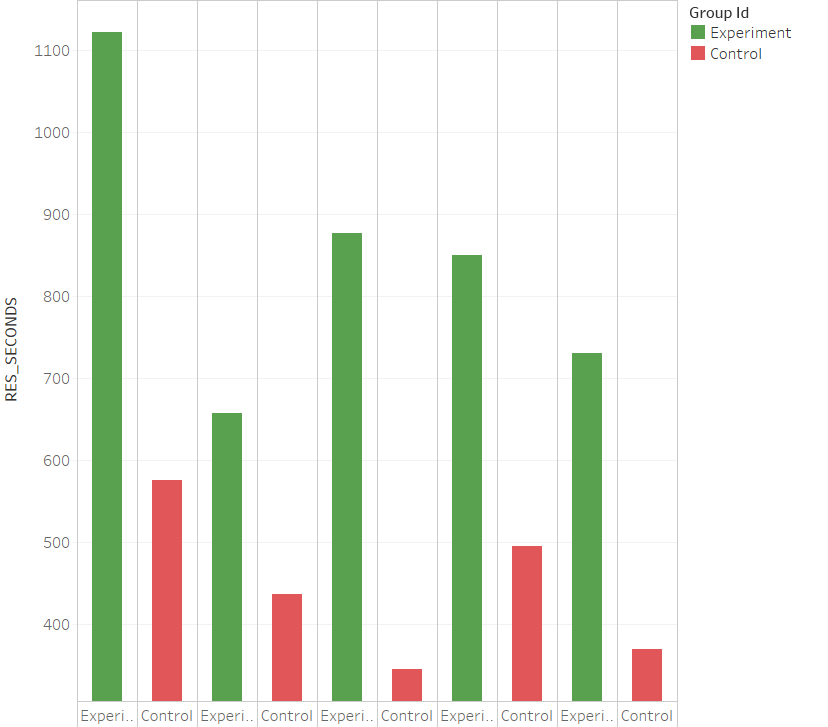
\includegraphics[width=0.9\textwidth]{DURATION_FILTERED}
    \caption{Duration of the warm up session.}
    \label{fig:durationOfWarmUp}
\end{figure}
\subsection{Heart Rate}
\begin{figure}[h]
    \centering
    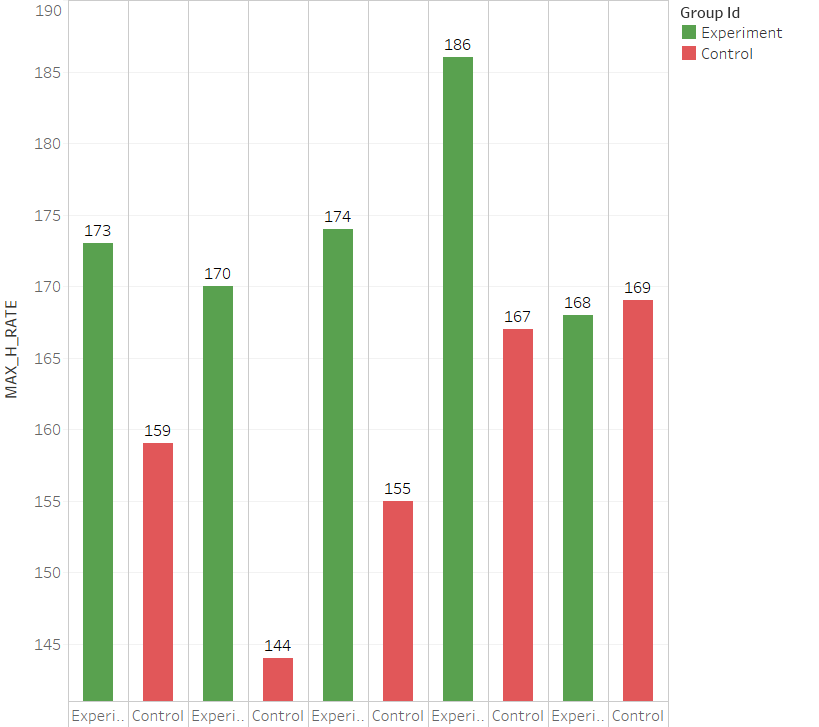
\includegraphics[width=0.9\textwidth]{MAX_HEART_RATE_FILTERED}
    \caption{Maximum heart rate for the participants.}
    \label{fig:heartRate}
\end{figure}
\subsection{Range of Motion}
\begin{figure}[h]
    \centering
    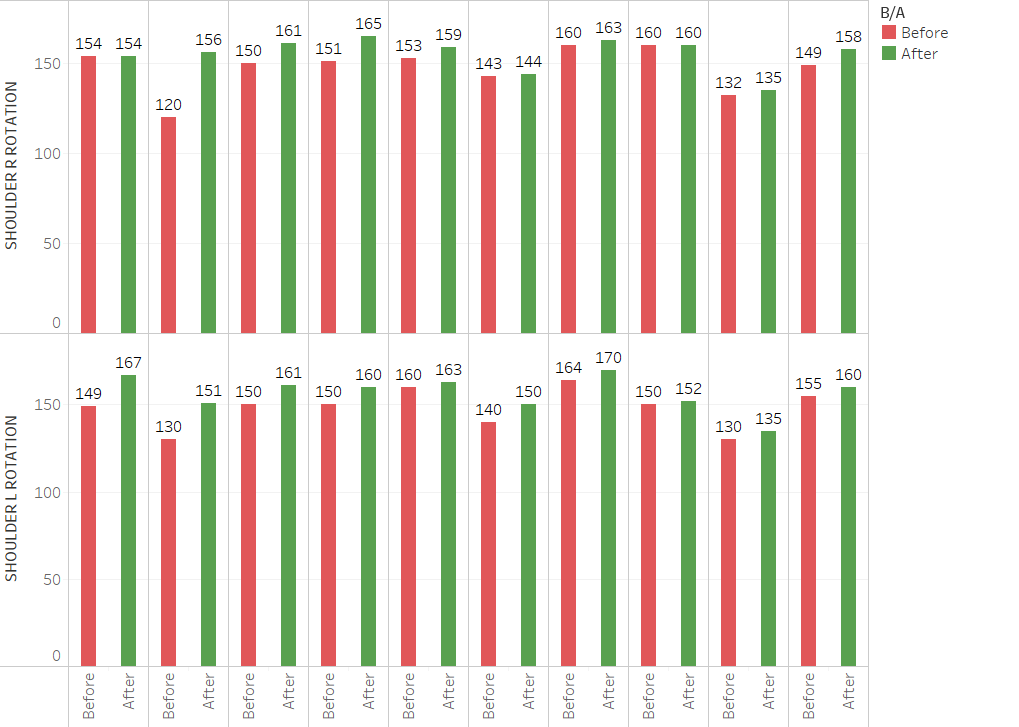
\includegraphics[width=0.9\textwidth]{SHOULDER_ROTATION}
    \caption{Shoulder rotation.}
    \label{fig:s_rot}
\end{figure}
\begin{figure}[h]
    \centering
    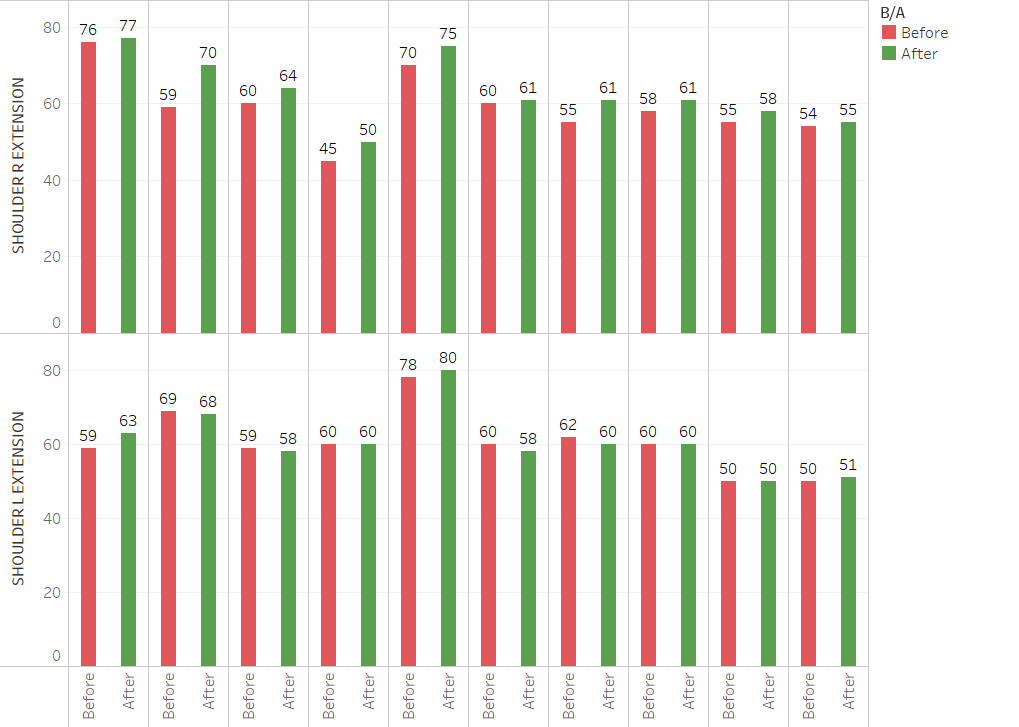
\includegraphics[width=0.9\textwidth]{SHOULDER_EXTENSION}
    \caption{Shoulder extension.}
    \label{fig:s_ext}
\end{figure}

\begin{figure}[h]
    \centering
    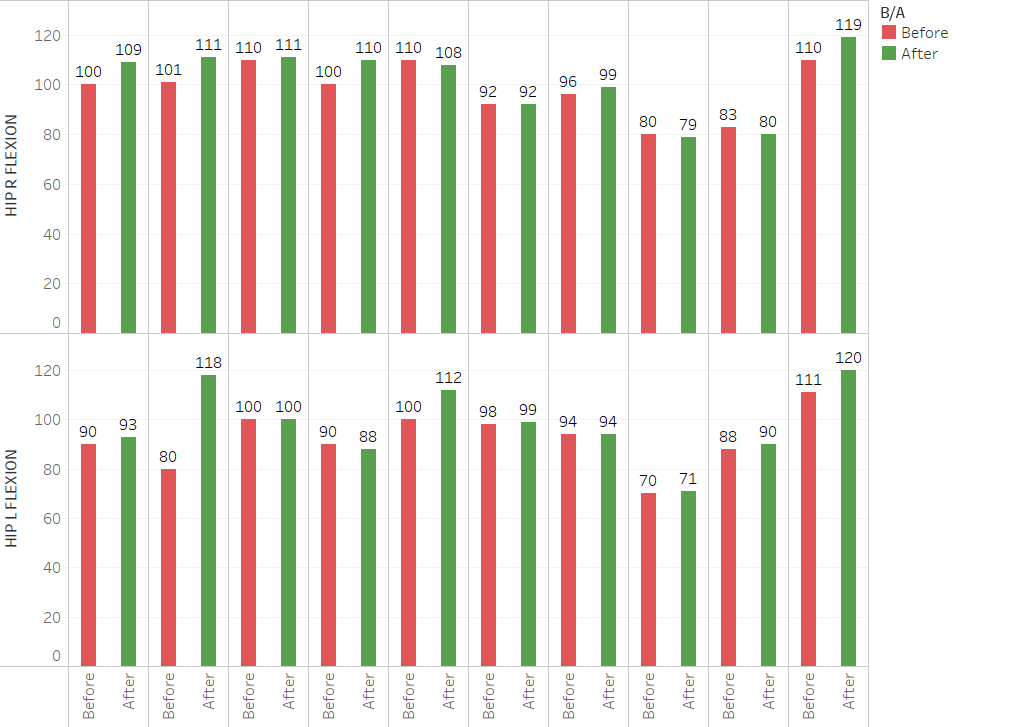
\includegraphics[width=0.9\textwidth]{HIP_FLEXION}
    \caption{Hip flexion.}
    \label{fig:h_flex}
\end{figure}

\begin{figure}[h]
    \centering
    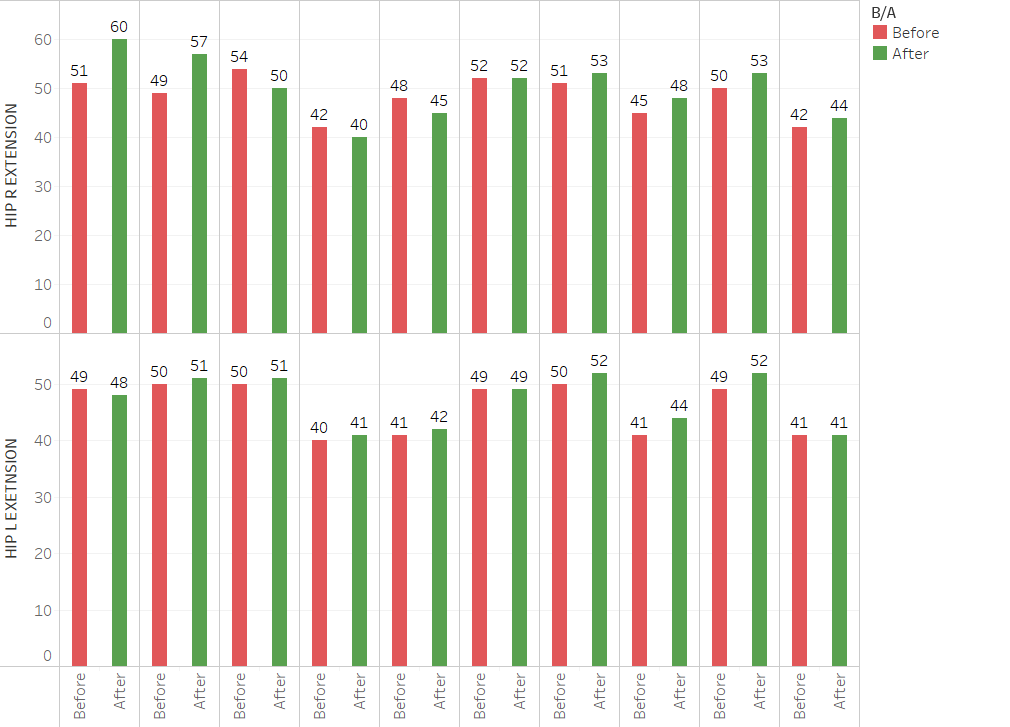
\includegraphics[width=0.9\textwidth]{HIP_EXTENSION}
    \caption{Hip extension.}
    \label{fig:h_ext}
\end{figure}